\documentclass{article}
\usepackage{graphicx} % Required for inserting images

\title{Bioinformatics Report}

\begin{document}

\maketitle

\section{Over-expression} %fabio
The first part of the project aims to predict the \textbf{overexpression} of the \textbf{BRCA1} gene. The starting point is feature vectors extracted using \textbf{UNI} from WSI of patients with breast cancer. Using the gene expression associated with our WSIs, we extracted a threshold that we need to construct our dataset. The task is related to a binary classification problem, where elements with a gene expression value below the threshold are assigned the label $0$, while those above are assigned the label $1$. The base models used in our experiments are \textbf{ABMIL} and \textbf{DSMIL}. We also added a model that we called \textbf{DS\_ABMIL}, which replaces the instance classifier of DSMIL with the attention calculation from ABMIL.
All experiments were conducted using a \textbf{Stratified K-fold} with K=5, \textbf{early stopping} with patience=5, 10 epochs, and the \textbf{CosineAnnealingLR} scheduler.

\subsection{ABMIL}
The first model tested is an implementation of ABMIL (cite the paper). First, we apply a linear layer to reduce the input dimensionality from $n\_patch \times 1024$ to $32$. Tests have shown that  is the optimal value for the  \textbf{inner\_dim} parameter. Subsequently, the following attention mechanism is applied:

\begin{equation}
	att = \frac{\exp\{W^\top \tanh(V h^\top) \odot \sigma(U h^\top)\}}{\sum_{j=1}^{n\_patch} \exp\{W^\top \tanh(V h_j^\top) \odot \sigma(U h_j^\top)\}} \quad
\end{equation}

where $U, V \in R^{ n\_patch \times inner\_dim}, w \in R^{n\_patch \times 1}$ are parameters, $\odot$ is an element-wise multiplication, and $\sigma(\cdot)$ is the sigmoid non-linearity.

Subsequently, two linear layers are applied to gradually reduce the dimensionality.
\subsubsection{Results}

\subsection{DSMIL}
The second model we used is DSMIL (cite the paper). As in the previous case, we first applied a linear layer to reduce the dimensionality of our patches. In this case, we do not observe a significant improvement in performance.
\begin{figure}[h]
	\centering
	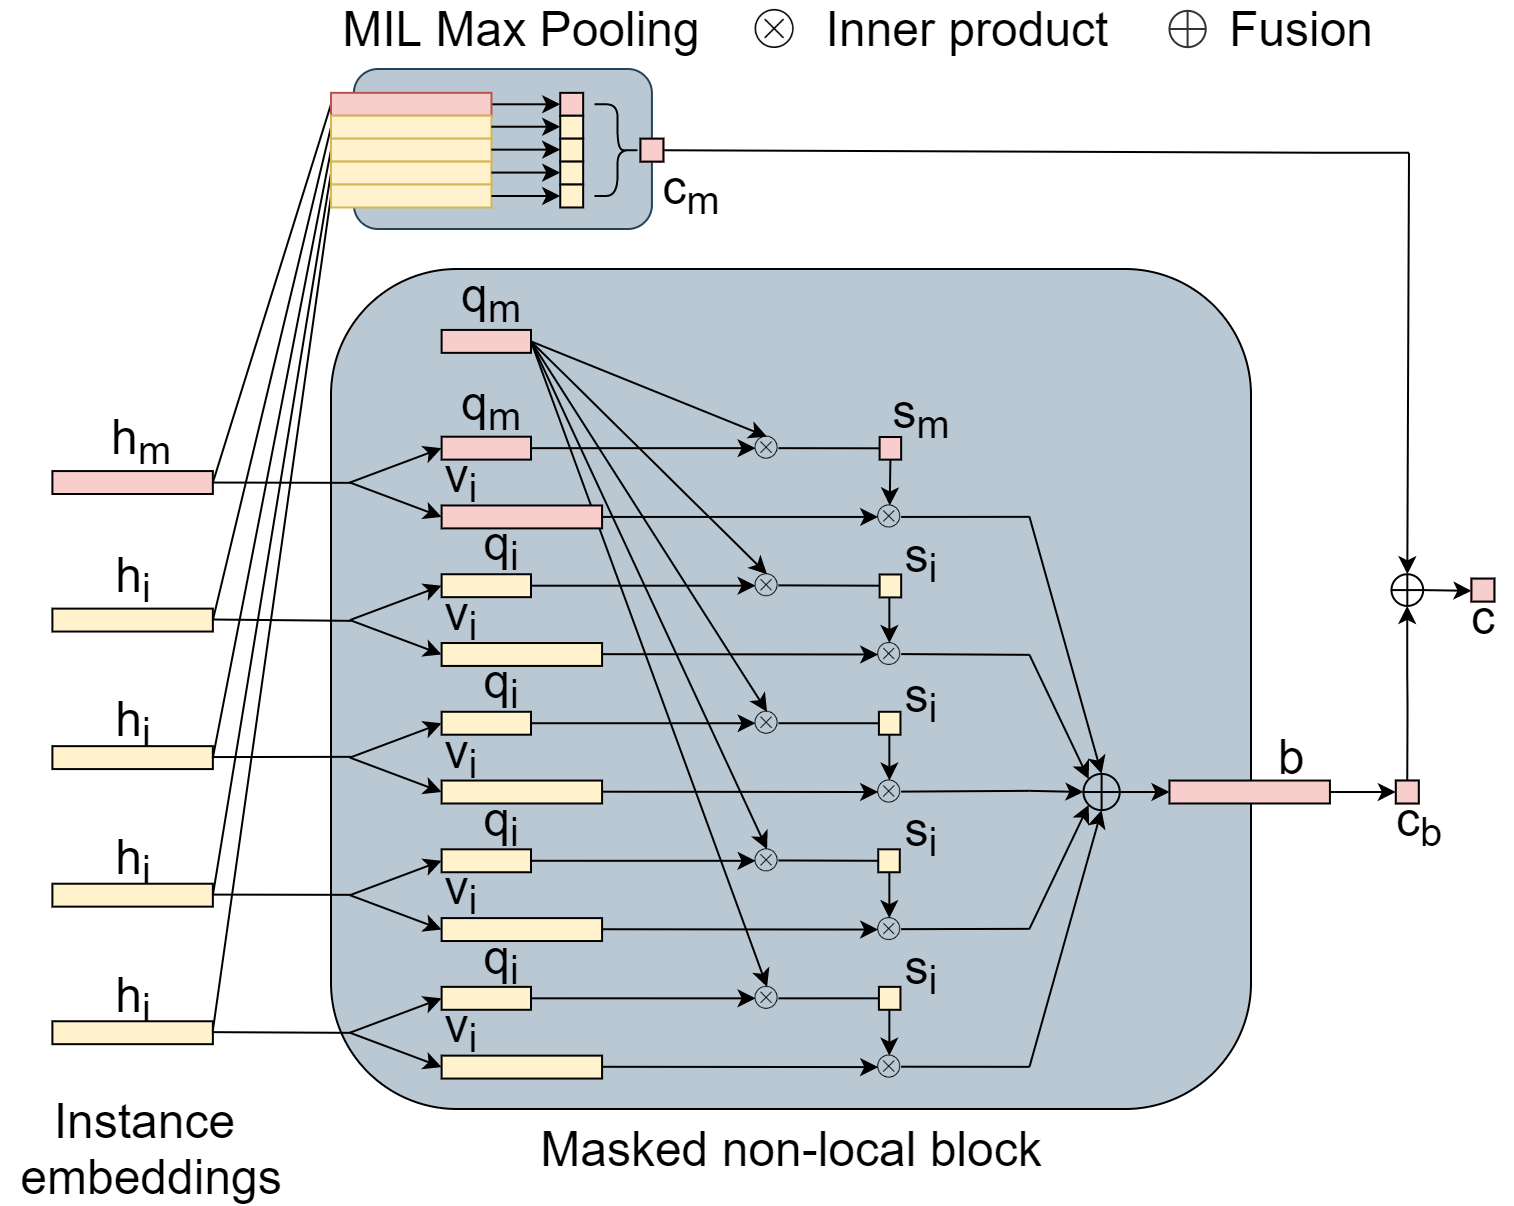
\includegraphics[width=0.8\textwidth]{images/dsmil.png}
	\caption{DSMIL model scheme}
\end{figure}

\subsubsection{Results}

\subsection{DS\_ABMIL}
This model is obtained by replacing the instance classifier of DSMIL with the attention calculation from ABMIL. The training of the model occurs in the same manner as DSMIL.

\subsubsection{Results}

\subsection{Comparison}

Prendi i migliori dei vari metodi.
Metti anche parentesi regressione


\section{Attention Map} %fabio
The ultimate goal of our project is to visualize attention maps that provide an explanation for the decisions made by the model. The models we tested utilize whole slide images (WSI) represented through UNI features with a shape of $n\_patch\times1024$. What we have done is overlay a heat-map representing the importance of each patch onto a reduced version of the WSI.
This process is composed by two steps:
\begin{itemize}
	\item compute the attention on the single patch
	\item compute the activation map of each patch
\end{itemize}

Add block scheme

\subsection{Patch-level attention}

Starting from the identifier of a WSI, we can input it into our model to obtain the desired classification as well as the attention for each individual patch. The attention scores are normalized and overlaid onto a reduced version of the WSI to identify which patches are the most important.

\begin{figure}[h]
	\centering
	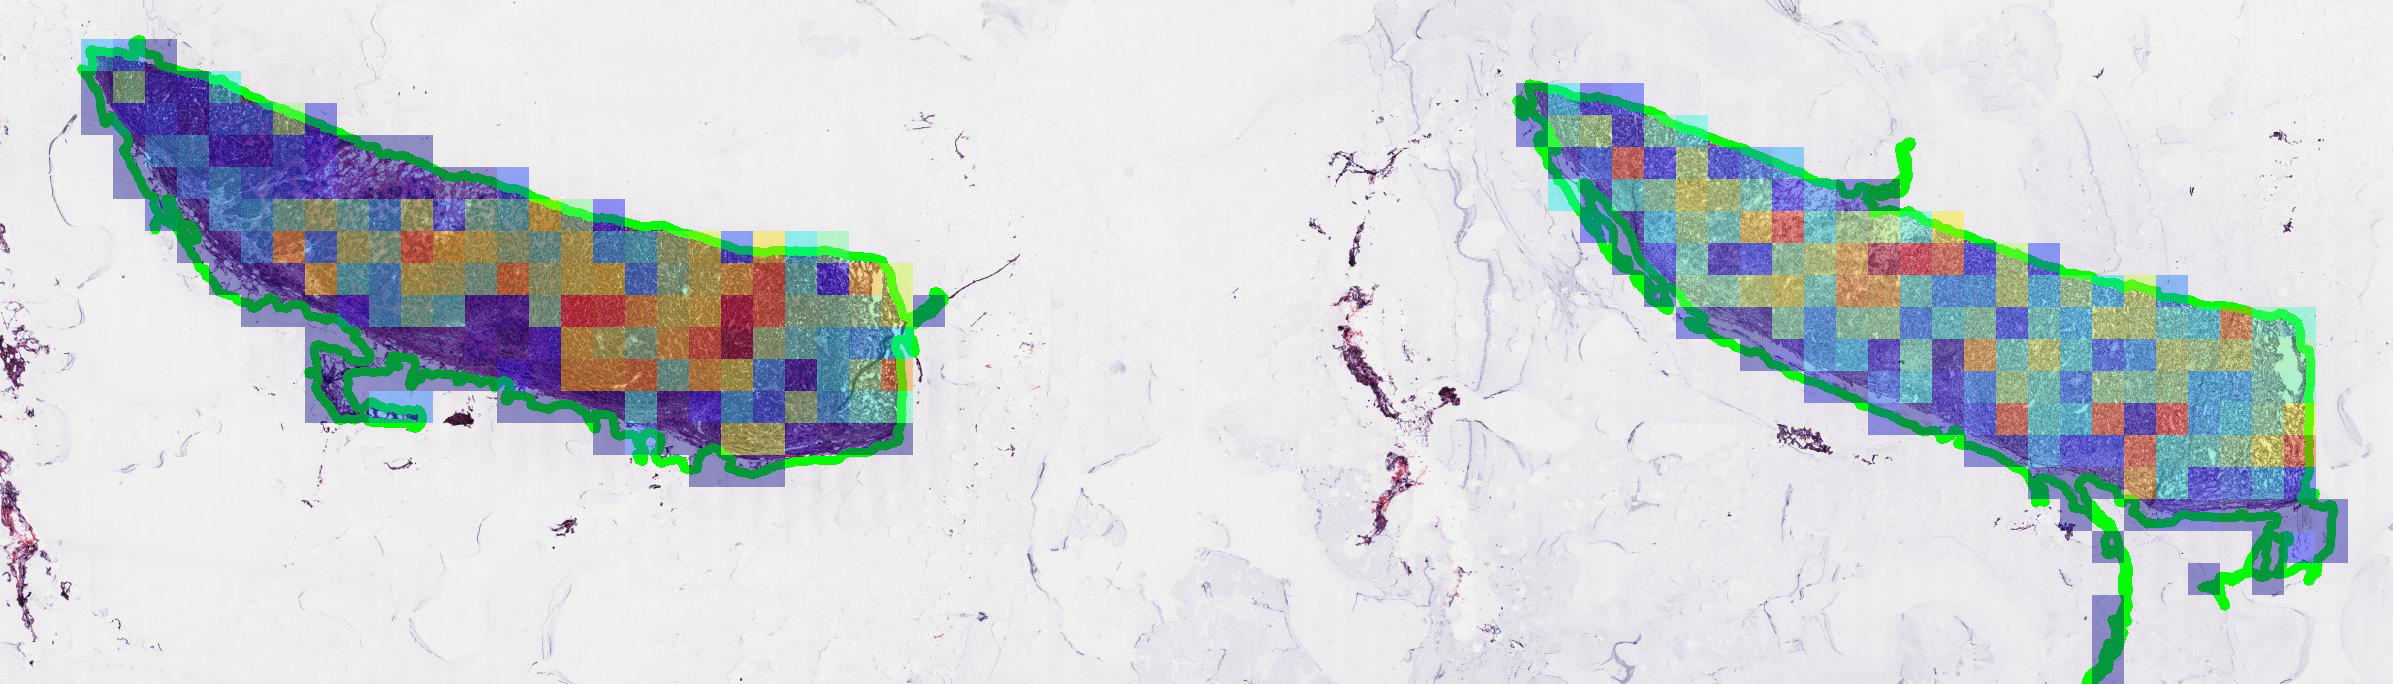
\includegraphics[width=1\textwidth]{images/old_attention_map_val.png}
	\caption{Patch-level attention projected on to the WSI. Warmer colors means higher importance}
\end{figure}


\subsection{Inner patch attivation}
We have introduced this step to obtain an attention map that also considers the importance of the elements within each individual patch. Each patch, which has a size of $1024\times1024$, is resized to $224\times224$ and subsequently passed through a ResNet50. This is done to obtain the activation map.

For each patch, we multiply the normalized activation map by the normalized attention value obtained in the previous step. In this way, we generate a heat-map to overlay on the image that takes into account both the importance of the patch in the decision of our model and the internal features of each patch.

Before being utilized, we applied a Gaussian filter with $\sigma =2$ to smooth the edges between the patches. Additionally, a threshold was applied to display only values that had scores exceeding $0.8$.
 
\begin{figure}[h]
	\centering
	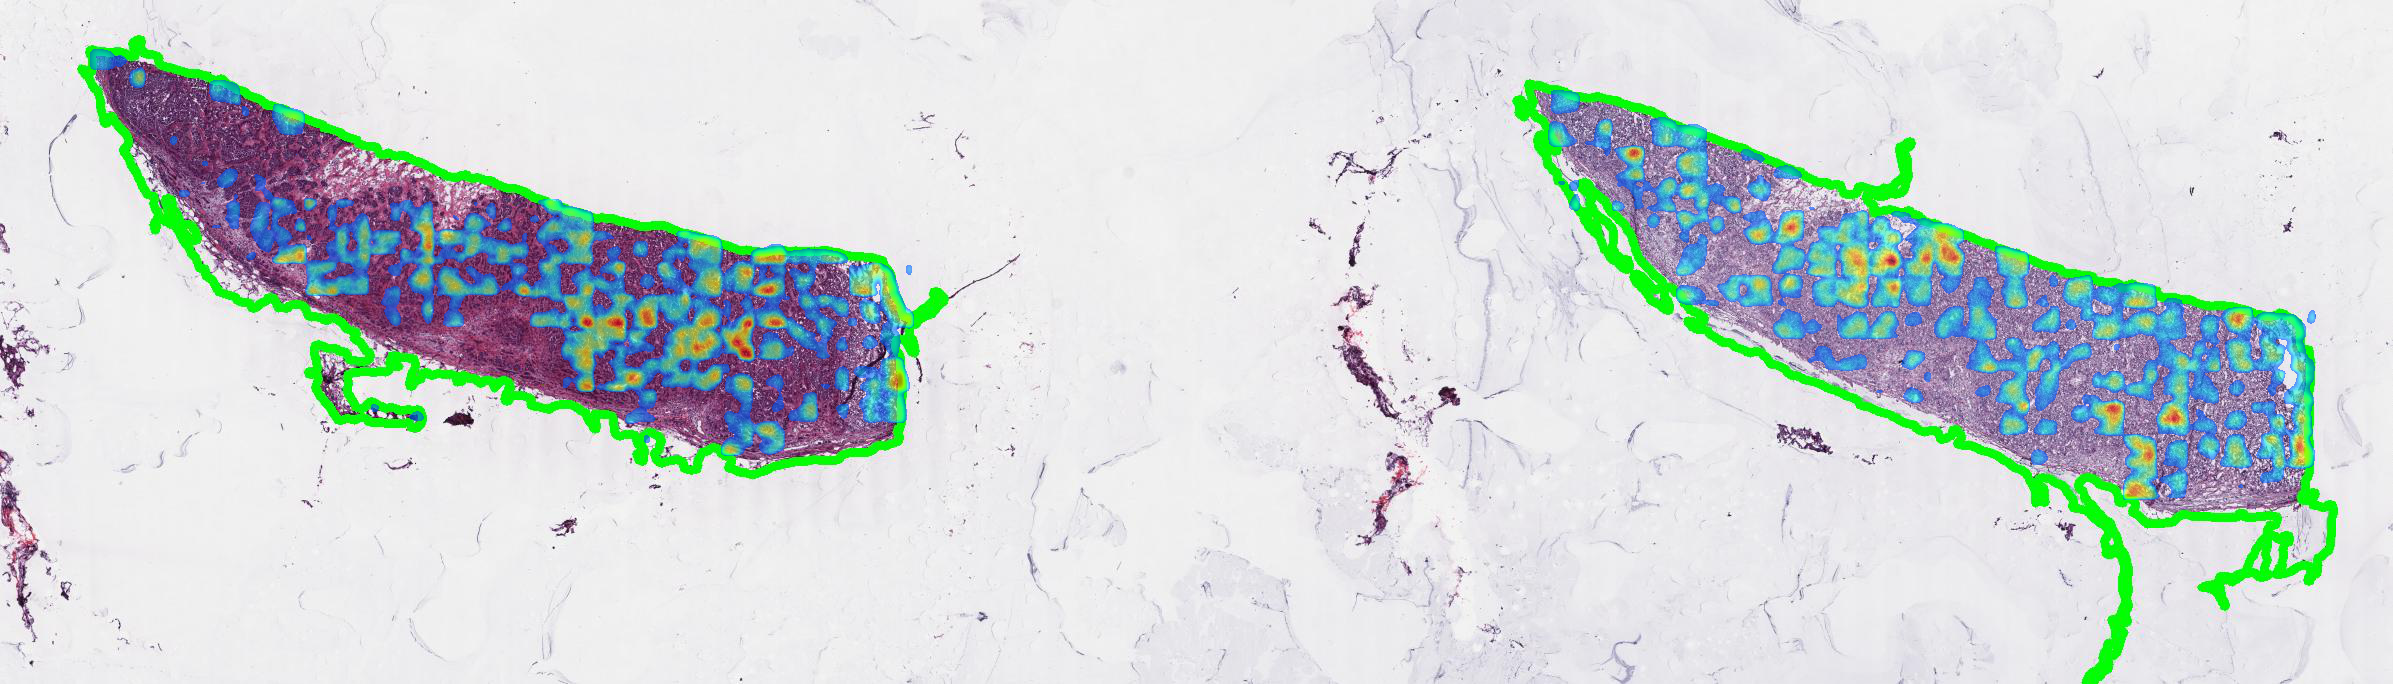
\includegraphics[width=1\textwidth]{images/attention_map_val.png}
	\caption{Final result that takes into account patch-level attention and inner patch features}
\end{figure}

\newpage

\end{document}